\documentclass{article}
\usepackage[utf8]{inputenc}
\usepackage[maxcitenames=1,style=numeric]{biblatex}
\usepackage{amsmath}
\usepackage{amssymb}
\usepackage{amsthm}
\usepackage{tcolorbox}
\usepackage{graphicx}
\usepackage{algorithm}
\usepackage{algorithmic}
\usepackage{subfig}
\usepackage{hyperref}
\usepackage{cleveref}
\usepackage{thmtools}
\usepackage{thm-restate}
\usepackage{enumerate}
\usepackage{xcolor}

\title{Machine Learning based TIR predictor}
\author{u6015325 }
\date{\today{}}

\bibliography{ref.bib}
\DeclareUnicodeCharacter{2212}{-}
\begin{document}

\maketitle

\section{Introduction}

One of the main tenets of synthetic biology is design, evaluation and standardisation of genetic parts \cite{Brophy2014,Canton2008,Stanton2014}. This can be done in variety of ways, most of each involve designing the DNA sequence in CAD software and then physically testing it in a laboratory. Alternative to this is computer modelling and prediction of part behaviour based on the designed DNA sequence or design of DNA sequence based on expected function \cite{Yeoh2019,Nielsen2016}. Most of these models are based on either the thermodynamic properties of the involved molecules (DNA, RNA, proteins among others) or empirically obtained values describing a relevant to design value, like Translation Initiation Rate (TRI) in case of Ribosome Binding Sites (RBS) \cite{Xia1998,Chen2013,Reeve2014}.\\
According to Reeve \emph{et al.} there are three main RBS calculators, all predicting the TRI based on the thermodynamic properties of the RBS and the ribosome \cite{Seo2013,Na2010,Salis2009}. Predictions from all of these models are relatively good ($R^2 >0.8$), there come with a number of caveats: i) they rely on calculations of free energies that can be hard to calculate ii) in general, the models' accuracy is improved by increasing the number of phenomenons taking place during the translation, but this can lead to paradoxically decreased model accuracy due to accumulation of errors \cite{EspahBorujeni2016} and iii) by using deterministic coefficients to calculate energies one disregards often stochastic nature of processes in the cells which again increases perceived prediction error \cite{Goss1998}. \\
Synthetic biology is currently going through a phase of exponential increase in volume of data produced during experiments. \cite{Freemont2019} New experimental methods heavily relying on advances in automation and microfludics allow unprecedented precision and throughput in data generation. These new data-sets can be combined with data reliant machine learning algorithms to generate new models and predictors for use in synthetic biology \cite{Camacho2018}. In the past few years there was a significant uptick of Machine Learning based approaches to synthetic biology. Jervis \emph{et al.} used support vector machine and neural network to optimise production of monoterpenoid in \emph{Esherichia coli} \cite{Jervis2019}. Similarly, Costello \emph{et al.} have used a number of machine learning approaches to analyse time-series multiomics data to predict metabolic pathway bahaviour \cite{Costello2018}. There were also successful attempts at using deep learning techniques for analysis of big data-sets \cite{Alipanahi2015,Angermueller2016}. However, the use of machine learning in synthetic biology is still in its infancy and will require additional research to show its full potential. \\
Here we present a machine learning workflow for building a RBS translation rate predictor based on fluorescence data from cultures. RBS being one of the key genetic elements controlling protein expression and at he same time having a relatively short sequence is a perfect target for establishing workflows that can be later translated to more complicated systems. We have used Gaussian Process-Upper Confidence Bound and Bandits algorithms to analyse and optimise the initiation rates of the designed RBS.

\section{Genetic device design}
There is a number of qualities that impact the translation rate, but chief among them are concerned with how the ribosome recognises and binds to the RBS sequence \cite{Chen1994,Vellanoweth1992}. In \emph{E. coli} the RBS is usually located in the 20 bases downstream of the start codon. The RBS usually has a distinguishable, consensus, core sequence called the Shine-Dalgarno sequence, which in \emph{E. coli} is AGGAGG. Here, we put that 20 bp long sequence into focus with main emphasis being put on the 6bp core region (Figure 1).\\
The RBS controls expression of the Green Fluorescent Protein (GFP) in its mut3b variant. By controlling expression of a fluorescent protein with the RBS we can quickly assess the perceived TIR by measuring fluorescence of cells harbouring the device. Finally, the mRNA is transcribed from an IPTG-inducible promoter pLlacO-1. By making the whole device inducible we can synchronise the start of the expression of the GFP in all the cultures by inducing them at the same optical density (OD\textsubscript{600}) with addition of IPTG.\\


\begin{figure}[t]
    \centering
    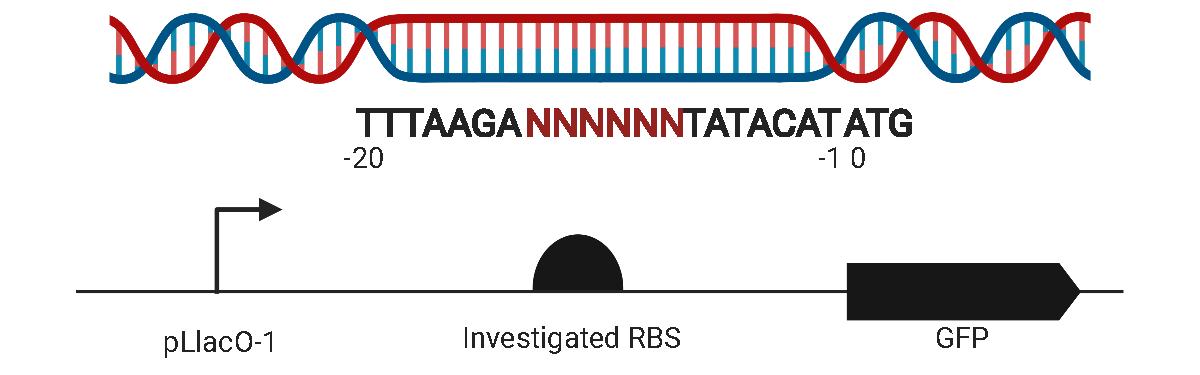
\includegraphics[scale=0.6]{plots/RBS_anatomy.pdf}
    \caption{\textbf{Diagram of the investigated sequence.} The sequence of the investigated RBS is shown with the randomised core sequence in red. The start codon of the GFP coding sequence is also shown with numbers showing relative nucleotide positions. At the bottom a simplified SBOL diagram of the genetic device is shown.}
    \label{fig: Anatomy of the randomized sequence.}
\end{figure}

\section{Methods}

\subsection{Plasmid Design}

We have used the pBbB6c-GFP plasmid for all our designs. This plasmid comes with GFP mut3b CDS inducible with addition of IPTG. The original RBS for the GFP CDS was replaced with combination of PCR and isothermal assembly. Primers and the assembly strategy have been generated using the Teselagen DESIGN software (Teselagen Biotechnology).

\subsection{PCR}
PCR amplification of the cloning inserts was done using Q5 High-Fidelity 2X Master Mix (NEB, catalogue no. M0492L). 20 \(\mu\)L reactions were prepared by dispensing each of the 10 \(\mu\)M reverse primers into a well of a 96-well PCR plate using the Labcyte Echo Liquid Handler. A mastermix consisting of polymerase premix, plasmid DNA template, and the single 10 forward primer was prepared by and dispensed by hand. Reactions were run using Touchdown PCR or standard PCR cycling methods in BioRad C1000 thermal cyclers. Then, samples were incubated at 37$^{\circ}$C for 60 minutes, followed by a 20-minute heat inactivation step at 80$^{\circ}$C.
Capillary electrophoresis of PCR products was performed using the Agilent Technologies ZAG DNA Analyzer system. 2\(\mu\)L of each PCR reaction was electrophoresed using the ZAG 130 dsDNA Kit (75-20000bp) or ZAG 110 dsDNA Kit (35-5000bp) (Agilent Technologies, catalogue no. ZAG-110-5000; ZAG-130-5000). ProSize Data Analysis Software (Agilent Technologies) was used to generated gel images from the sample chromatograms and sizes were estimated by reference to the upper and lower DNA markers spiked into each sample and a DNA ladder run in well H12 of each sample plate. 

\subsection{Isothermal DNA Assembly}
Constructs were assembled using NEBuilder HiFi DNA Assembly Master Mix (NEB, catalogue no. E2621L). Samples were incubated at 37$^{\circ}$C for 60 minutes, followed by a 20-minute heat inactivation step at 80$^{\circ}$C. Reactions consisting of the common fragment and the variable fragment were prepared using the Echo acoustic liquid handler, to a final volume of 5 or 10\(\mu\)L . Assemblies were run in the thermal cycler for 1 hour at 50$^{\circ}$C, followed by an infinite hold step at 4$^{\circ}$C.

\subsection{\textit{E. coli} transformation}
The DH5α cell line (Thermo Fisher Scientific, catalogue no. 18265017) was made chemically competent using the Mix & Go \textit{E. coli} Transformation Kit & Buffer Set (Zymo Research, catalogue no. T3001). 20\(\mu\)L of cells was aliquoted into each well of a cold 96-well PCR plate and stored at -80$^{\circ}$C for later use. Plates of cells were thawed on a -20$^{\circ}$C cold block before 3µL of the assembly product was added and mixed using the CyBio FeliX liquid handler. Cells were incubated on a cold block for 2-5 minutes before being plated in a 96 square grid on Omnitrays containing LB (BD, catalogue no. ***) with 34\(\mu\)g/mL chloramphenicol (Sigma, catalogue no. ***). Multiple dilutions of cells in LB were prepared and plated in parallel on Omnitrays in 96 square grid. Plates were incubated overnight at 37$^{\circ}$C.

\subsection{Automated colony picking and culturing}
A Singer Instruments PIXL colony picker was used to select individual colonies from the transformation plates. Each selected colony was used to inoculate 1mL of selective medium in a 2mL square well 96 plate. They were then cultured overnight in 37$^{\circ}$C with shaking (~300rpm).

\subsection{Glycerol stock preparation}
100\(\mu\)L of sterile 80\% (v/v) glycerol and 100\(\mu\)L of overnight culture were combined in the wells of a 96 deep (2mL) round well plate using the CyBio Felix liquid handler. They were then sealed with a 96-well silicon sealing mat and transferred to a -80$^{\circ}$C freezer. 

\subsection{Cuture analysis}
Overnight cultures were started by inoculating 1mL of LB medium supplemented with 34\(\mu\)g/mL chloramphenicol with ~2\(\mu\)L of the glycerol stock in a 96 deep (2mL) round well plate. Cultures were incubated at 37$^{\circ}$C with shaking (~300rpm) for ~17 hours. The following morning, 20\(\mu\)L of overnight culture was added to 980\(\mu\)L of fresh selection medium and precultures were grown at 37$^{\circ}$C with shaking in 2mL round well 96 plate. 
After 90 minutes, two parallel cultures were prepared in flat-bottom clear polystyrene 96-well plates and were induced with 500\(\mu\)M IPTG – one plate of 300\(\mu\)L cultures for flow cytometry analysis (induced with 1.5\(\mu\)L of 0.1M IPTG) and one plate of 200\(\mu\)L cultures for plate reader analysis (induced with 1.0\(\mu\)L of 0.1M IPTG).
•	Cytation 5 acquisition and incubation/shaking settings
•	CytoFLEX S acquisition settings

\subsection{Machine learning experimental design}

To automatically design the RBS sequences in batch using machine learning, we consider two parts: 
1) Design an regression algorithm which takes the RBS sequences as input and returns the predicted TIR scores and the confidence intervals. 
2) Design an online learning approach which recommends the RBS sequences based on the predicted TIR scores and confidence intervals. 
Such online learning approach provides the $\textit{exploitation-exploration balance}$ that we use to control our machine learning process.

With the goal of finding RBS sequences with the largest possible TIR score after a total number of rounds $N$,  we consider our experimental design problem as sequentially optimising an unknown reward function $f: \mathcal{D} \rightarrow \mathbb{R}$, where $\mathcal{D}$ is the set containing all RBS sequence points, and $f(\mathbf{x})$ is the TIR score at $\mathbf{x}$. 
In each round $t$, we choose a set of $m$ points $\mathcal{S}_t \subset \mathcal{D}$ and observe the function values of each points in the selected set $\mathcal{S}_t$, i.e. $y_i = f(\mathbf{x}_i) + \epsilon_i$, for all $i \in \mathcal{S}$, where $\epsilon_i$ is the noise (we assume the noise is following Gaussian distribution with unknown mean and variance). This noise is influenced by the accuracy of the RBS predictor and other experimental interference (e.g. time, temperature, operator, etc.). 

For regression model, we consider the \textit{Gaussian Process Regression (GPR)}.
A Gaussian process regression model \cite{Rasmussen2004} is a Bayesian approach which provides uncertainty measurements on predictions. 
We model $f$ as a sample from a \textit{Gaussian process} $\mathcal{G} \mathcal{P}(\mu(\mathbf{x}), k(\mathbf{x}, \mathbf{x'}))$, which is specified by the mean function $\mu(\mathbf{x})=\mathbb{E}[f(\mathbf{x})]$ and the kernel (or covariance) function $k\left(\mathbf{x}, \mathbf{x}^{\prime}\right)=\mathbb{E}[(f(\mathbf{x})-\left.\mu(\mathbf{x}))\left(f\left(\mathbf{x}^{\prime}\right)-\mu\left(\mathbf{x}^{\prime}\right)\right)\right]$.
Denote the training testing data as $X, X_{*}$, and the training label as $\mathbf{y}$.
Then the posterior of the test points (i.e. predictive distributions) is given by the conditional distribution $\mathbf{f}_\ast | X, \mathbf{y}, X_\ast \sim \mathcal{N}(\bar{\mathbf{f}}_\ast, cov(\mathbf{f}_\ast))$, where
\begin{align}
\overline{\mathbf{f}}_{*} & \triangleq \mathbb{E}\left[\mathbf{f}_{*} \mid X, \mathbf{y}, X_{*}\right]=K\left(X_{*}, X\right)\left[K(X, X)+\alpha^{2} I\right]^{-1} \mathbf{y} \\
\label{Eq: predicted variance in main paper}
\operatorname{cov}\left(\mathbf{f}_{*}\right) &=K\left(X_{*}, X_{*}\right)-K\left(X_{*}, X\right)\left[K(X, X)+\alpha^{2} I\right]^{-1} K\left(X, X_{*}\right) 
\end{align}
%For noisy test targets $\mathbf{y}_\ast$, we can compute the predictive distribution by adding $\alpha^2 I$ to the variance term $cov(\mathbf{f}_\ast)$ in Eq. (\ref{Eq: predicted variance in main paper}).

To represent the RBS sequences and formulate the similarity between sequences, we use the \textit{weighted degree kernel with shift} \cite{ratsch_rase_2005} to specify the kernel function of $GP$.  
The weighted degree kernel with shift extends the spectrum kernel \cite{leslie2001spectrum, ben2008support} 
by considering the positional information and allowing some positional shifts of matching substrings.
The spectrum kernel and the weighted degree kernel with shifts are string kernels, which take two sequences as inputs and outputs a scalar value which represents the similarities between the two sequences. 
We define spectrum kernel firstly,
\begin{align}
        k_\ell^{\text{Spec}}(\textbf{x}, \textbf{x}^\prime) =\left\langle\phi_{\ell}^{\mathrm{Spec}}(\mathbf{x}), \phi_{\ell}^{\mathrm{Spec}}\left(\mathbf{x}^{\prime}\right)\right\rangle = \phi_{\ell}^{\mathrm{Spec}}(\mathbf{x})^T \phi_{\ell}^{\mathrm{Spec}}\left(\mathbf{x}^{\prime}\right).
    \end{align}
 where $\mathbf{x}, \mathbf{x}^\prime$ are two RBS sequences in $\mathcal{D}$ over an alphabet $\Sigma$. We denote the number of letters in the alphabet as $|\Sigma|$. 
$\phi_{\ell}^{\mathrm{spec}}(\mathbf{x})$ maps the sequence $\textbf{x}$ into a $|\Sigma|^\ell$ dimensional feature space, where each dimension is the count of the number of one of the $|\Sigma|^\ell$ possible strings $s$ of length $\ell$. 
Let $X, X^\prime$ be two metrics which include $n$ sequences, and $\Phi_d^{Spec}(X) \in \mathbb{R}^{n \times |\Sigma|^{\ell}}$, then the spectrum kernel over metrics is 
    \begin{align}
         K_\ell^{\text{Spec}}(X, X^\prime) = \Phi_{\ell}^{\mathrm{Spec}}(X) \Phi_{\ell}^{\mathrm{Spec}}\left(X^{\prime}\right)^T.
    \end{align}
The weighted degree kernel with shift is defined upon the spectrum kernel, with flexibility of adjusting the substring length $d$, the start position $l$ and the shift length $s$. WDS kernel counts the match of kmers at corresponding positions in two sequences as shown in the following,
\begin{align}
        k_\ell^{WDS}(\mathbf{x}, \mathbf{x}^\prime) 
        &= \sum_{d=1}^{\ell} \beta_d \sum_{l=1}^{L-d+1} \gamma_l \sum_{s = 0, s + l \leq L}^{S(l)} \delta_s
        \left(k_d^{Spec}(\mathbf{x}_{[l+s:l+s+d]}, \mathbf{x}_{[l:l+d]}^\prime) + (k_d^{Spec}(\mathbf{x}_{[l:l+d]}, \mathbf{x}_{[l+s:l+s+d]}^\prime)\right)\\
        &= \sum_{d=1}^{\ell} \beta_d \sum_{l=1}^{L-d+1} \gamma_l \sum_{s = 0, s + l \leq L}^{S(l)} \delta_s
        \left(\mathbb{I}(\mathbf{x}_{[l+s:l+s+d]} = \mathbf{x}_{[l:l+d]}^\prime) + (\mathbb{I}(\mathbf{x}_{[l:l+d]}= \mathbf{x}_{[l+s:l+s+d]}^\prime)\right),
\end{align}
where $\beta_d = \frac{2(\ell - d + 1)}{\ell(\ell+1)}, \delta_s = \frac{1}{2(s+1)}$, $\gamma_l$ is a weighting over the position in the
sequence, where we choose to use a uniform weighting over the sequences, i.e. $\gamma_l = 1/L$. $S(l)$ determines the shift
range at position $l$. 
%Since the sequences in provided data have the pattern that the core area is different from each other, and other areas are similar. So the kernel for Gaussian Process we are using is the sum of kernels, for core areas we use spectrum kernel with string as input directly, and for other areas we use one-hot encoding and dot product kernel for simplicity.
    
    
%  For recommendations, we consider the \textit{Upper Confidence Bound (UCB)} type algorithms. 
%  As one popular type of the bandit algorithms \cite{lattimore2018bandit}, the UCB type of algorithms are based on the \textit{optimism in the face of uncertainty},
 %provide various approaches to sequential design where an agent adaptively chooses one or more options among several actions based on certain policies. In our work we used the Upper Confidence Bound version of that algorithm, which is based on the \textit{optimism in the face of uncertainty}. The UCB algorithm, as the name suggests,
%  which basically select RBS sequences with the maximum upper confidence bound constructed by the sum of the predicted mean and $n$ standard deviation ($n > 0$), i.e. $\operatorname{argmax}_{\mathbf{x}_i \in \mathcal{D}} \left( \mu_t(\mathbf{x}_i) + \beta_t \sigma_t(\mathbf{x}_i)\right)$,
%     where $\beta_t$ is a hyperparameter balancing the exploitation and exploration, 
%     $\mu_t(\mathbf{x}_i), \sigma_t(\mathbf{x}_i)$ are the predicted mean and standard deviation at round $t$ for the sequence $\mathbf{x}_i$. 

For recommending RBS sequences to label, we consider the Upper Confidence Bound (UCB) algorithm, 
%which is based on the \textit{optimism in the face of uncertainty}, 
selecting RBS sequences with the maximum upper confidence bound at round $t$, i.e.
\begin{align}
\label{Eq: GPUCB}
    \operatorname{argmax}_{\mathbf{x}_i \in \mathcal{D}} \left( \mu_{t-1}(\mathbf{x}_i) + \beta_t \sigma_{t-1}(\mathbf{x}_i)\right),
\end{align}
where $\beta_t$ is a hyperparmeter balancing the exploitation and exploration, 
$\mu_t(\mathbf{x}_i), \sigma_t(\mathbf{x}_i)$ are the predicted mean and standard deviation at round $t$ for the sequence $\mathbf{x}_i$.

Since labelling sequences is time-consuming, it is unrealistic to recommend sequence sequentially (i.e. one-by-one) and waiting for the label for each round.
Therefore we consider recommending sequences in batch and use Gaussian Process Batch Upper Confidence Bound (GP-BUCB) algorithm  \cite{desautels2012parallelizing}.
With batches of size $B$, the feedback mapping is then defined as $fb[t] = \lfloor(t-1) / B\rfloor B$, i.e. 
\begin{align}
    \mathrm{fb}[t]=\left\{\begin{array}{cl}
    0 & : t \in\{1, \ldots, B\} \\
    B & : t \in\{B+1, \ldots, 2 B\} \\
    2 B & : t \in\{2 B+1, \ldots, 3 B\} \\
    & \vdots
    \end{array}\right.
\end{align}


A key property of Gaussian Process regression is that the predictive variance in Eq. (\ref{Eq: predicted variance in main paper}) only depends on observed points (i.e. features), but not on the labels of those observed points. 
So one can compute the posterior variance without actually observing the labels. 
The GP-BUCB policy is to select sequences that
\begin{align}
    \operatorname{argmax}_{\mathbf{x}_i \in \mathcal{D}} \left( \mu_{fb[t]}(\mathbf{x}_i) + \beta_t \sigma_{t-1}(\mathbf{x}_i)\right).
\end{align}
And only update $y_{t^{\prime}}=f\left(\boldsymbol{x}_{t^{\prime}}\right)+\varepsilon_{t^{\prime}} \text { for } t^{\prime} \in\{\mathrm{fb}[t]+1, \ldots, \mathrm{fb}[t+1]\}$ at the end of each batch ($\mathrm{fb}[t]<\mathrm{fb}[t+1]$). 
This is equivalent to sequential GP-UCB with \textit{hallucinated observations} $\boldsymbol{y}_{\mathrm{fb}[t]+1: t-1}=\left[\mu_{\mathrm{fb}[t]}\left(\boldsymbol{x}_{\mathrm{fb}[t]+1}\right), \ldots, \mu_{\mathrm{fb}[t]}\left(\boldsymbol{x}_{t-1}\right)\right]$, while the posterior variance decreases. 


\begin{figure}[t]
    \centering
    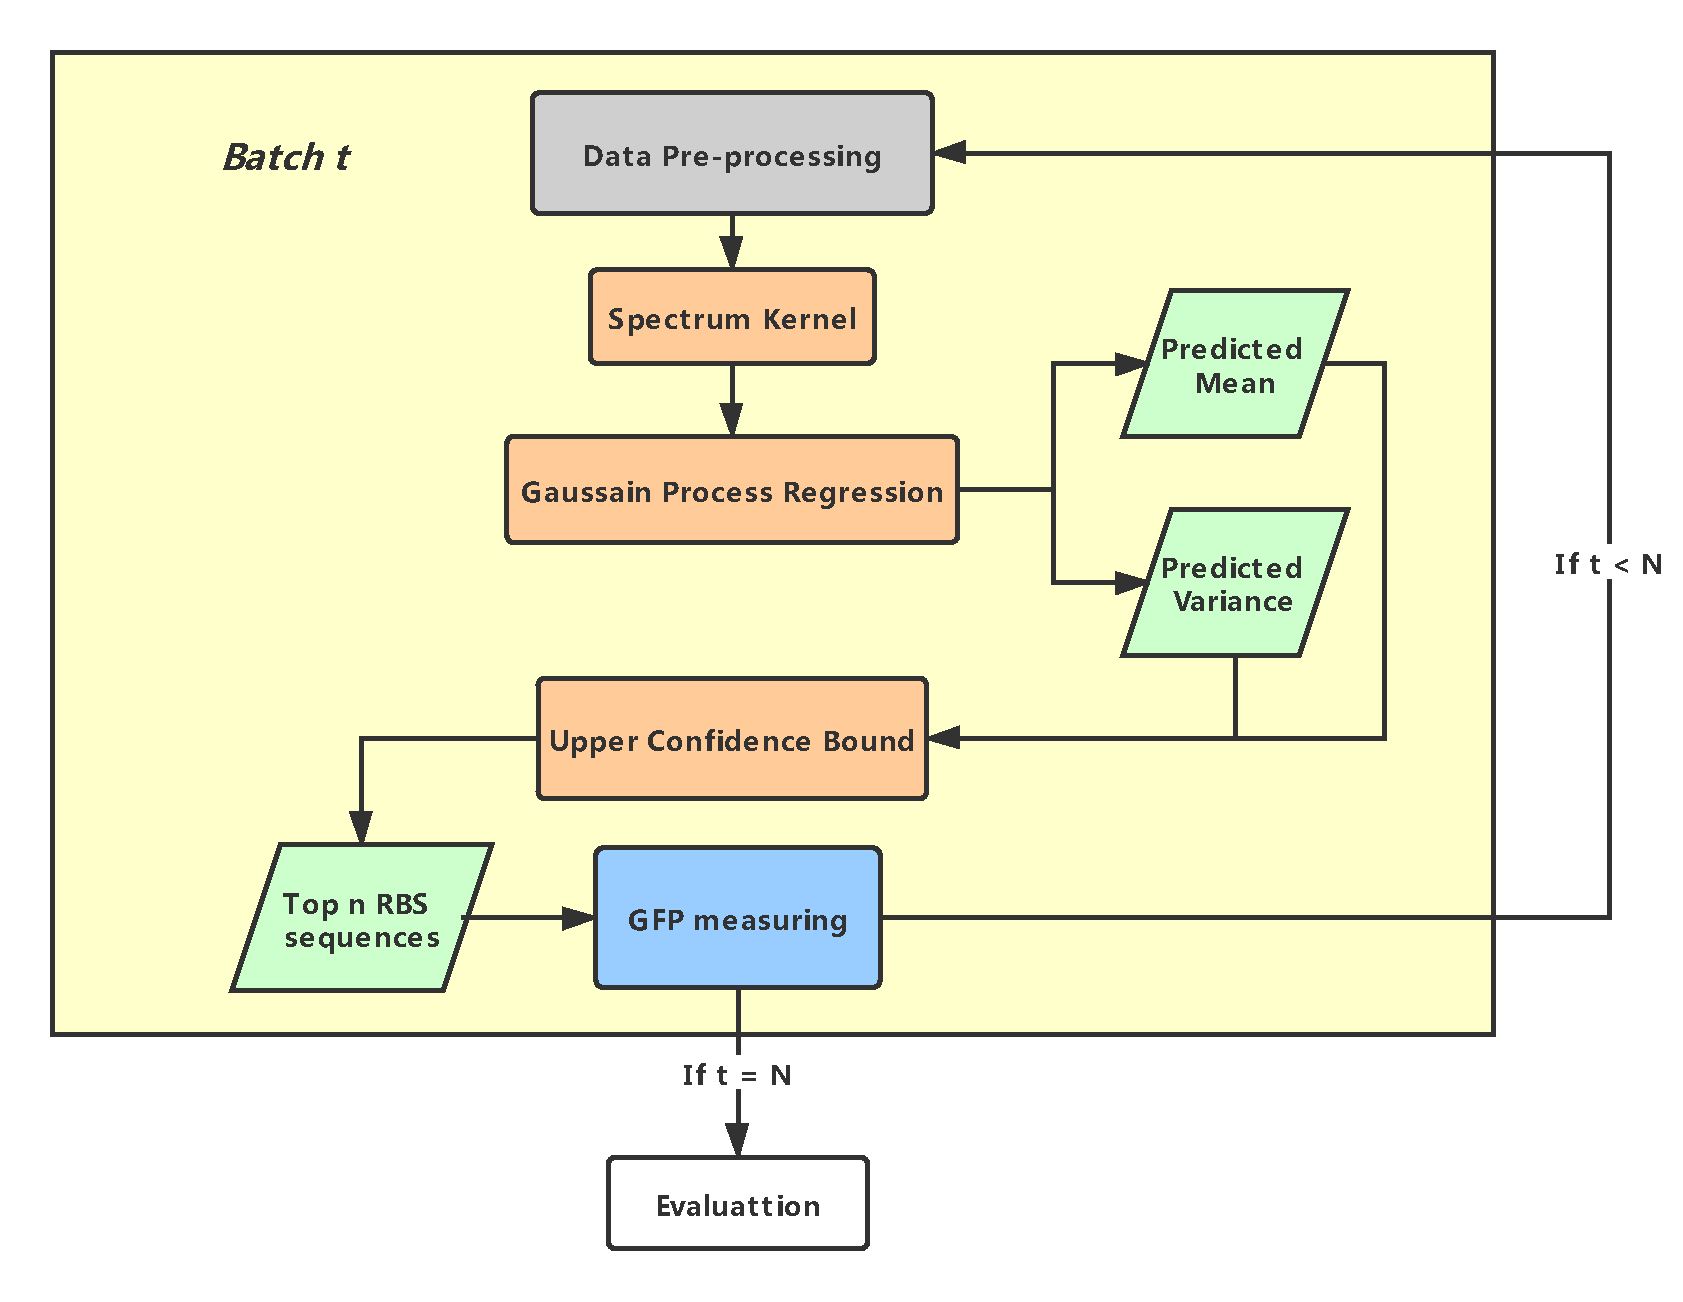
\includegraphics[scale=0.7]{plots/flowchart.pdf}
    \caption{Flowchart of machine learning based experimental design.}
    \label{fig: flowchart of machine learning based experimental design.}
\end{figure}







\section{Workflow Description}

Our experimental goal was to optimise the translation initiation rate by identifying the set of RBS sequences with top TIR scores with as fewer rounds as possible. We did this by designing a sequential experimental workflow, where we start with either randomised RBS sequences designed to explore the experimental space (round 1) or with RBS sequences recommended by the algorithm (subsequent rounds). The designs were then physically constructed in batches of 90 to fit our automated process (see \textbf{Methods} section). After constructing the plasmids harbouring the new devices are tested in microplate reader and flow cytometer. The results are then fed back to the algorithm for it to recommend the next round of designs.\\
The investigated RBS sequence is 20 bps long with the sequence TTTAAGAAGGAGATATACAT, which a known high TIR RBS that comes with the pBb series plasmids \cite{Lee2011}. In our design we focus on randomizing of the core -8 to -13 (relative to the GFP) bps of the RBS and fix others to be the same as the consensus sequence, i.e. TTTAAGA + NNNNNN + TATACAT. Since for each of the 6 position there are 4 possibilities: A, C, G, T the total feature space is $4^6$ = 4096.\\
For the first round of experiments, we design 180 (two times 90) RBS sequences based on the consensus sequence: 

\begin{enumerate}
    \item 60 RBS sequences which are subsequent single nucleotide changes of all 20 nucleotides of the original, consensus sequence. This batch is designed to show us influence of such single nucleotide changes on the overall performance of the RBS and the potential impact of changes made beyond the core part.
    \item 30 RBS sequences fully and uniformly randomised (equal probability of choosing either nucleotide for each position) 
    \item 30 RBS sequences randomised based on the position probability matrix (PPM) \textcolor{red}{we need a citation and better explanation for this}  
    \item 60 RBS sequences recommended by initial machine learning approach. For this, and subsequent design rounds, we use bandit optimisation algorithm called Gaussian Process Upper Confidence Bound (GPUCB) (see \textbf{Methods} section) \cite{srinivas2012information}. Since we don't have access to any prior data fitting our design we approximated the recommendations based on the data from \textcite{jervis2018machine}. This data contains 113 non-repeated records for 56 unique RBS sequences with the respective TIR label. The label values are between 0 - 100,000 and skewed, which is shown in Figure xx. We have normalised the label to 0 - 1 using the min-max normalisation.   
\end{enumerate}{}

\begin{figure}[t]
    \centering
    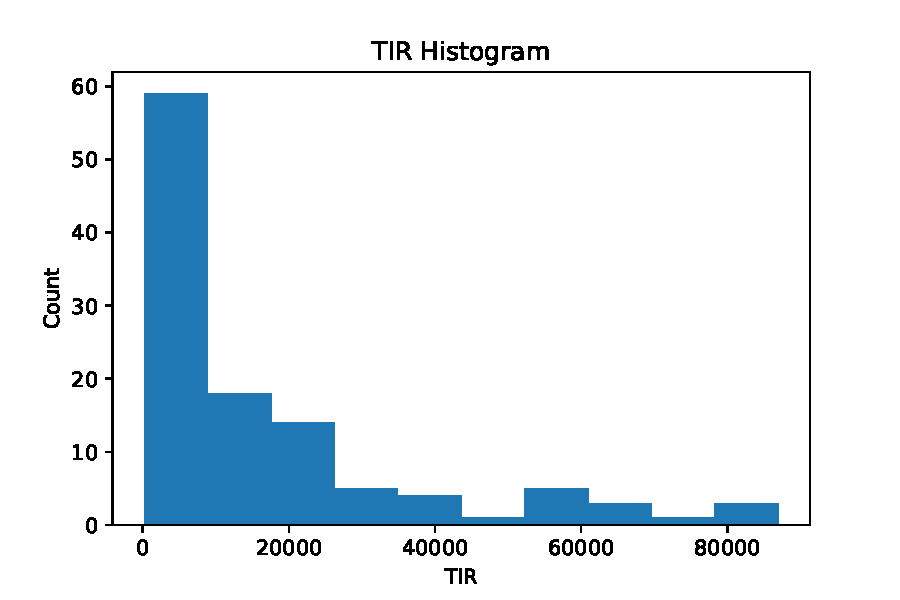
\includegraphics[scale=0.7]{plots/TIR_histogram.pdf}
    \caption{TIR Histogram.}
    \label{fig: TIR Histogram.}
\end{figure}

Based on the results from round one, we used the previously described algorithm to recommend another batch of 90 RBS. They have been then constructed and tested using the exact same methodology as the first round. In total, three more rounds have been performed, each with designs recommended by the algorithm. 

\section{Results}



\begin{enumerate}
    \item RMSE of predictions.
    
    \item Similarity of recommendations. 
    \begin{figure}[t]
    \centering
    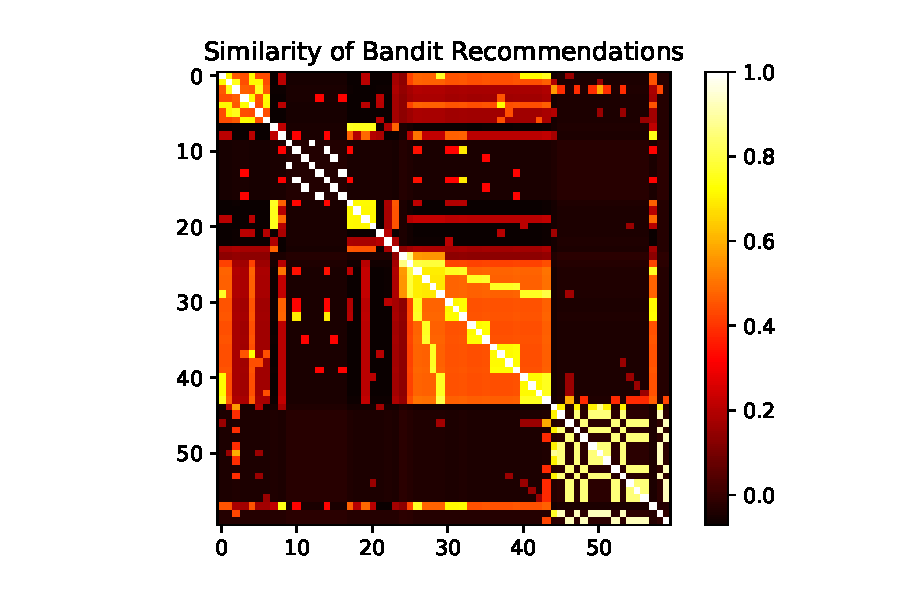
\includegraphics[scale=0.7]{plots/similarity_first_round_recommendation.pdf}
    \caption{TIR Histogram.}
    \label{fig: TIR Histogram.}
\end{figure}
\end{enumerate}{}


\newpage

\printbibliography
\end{document}
